\documentclass[conference]{IEEEtran}
\usepackage{amsmath,amssymb,amsfonts}
\usepackage{booktabs}
\usepackage{graphicx}
\usepackage{url}
\usepackage{microtype}
\usepackage{multirow}

\makeatletter
\newcommand{\linebreakand}{%
  \end{@IEEEauthorhalign}
  \hfill\mbox{}\par
  \mbox{}\hfill\begin{@IEEEauthorhalign}
}
\makeatother

\title{NeuralFabric: Capacity-Guarded Predictive Routing on a Synthetic Datacenter Fabric}

\author{
\IEEEauthorblockN{Divyank Seervi}
\IEEEauthorblockA{\textit{SCOPE}\\
\textit{VIT Vellore}\\
divyank.seervi2024@vitstudent.ac.in}
\and
\IEEEauthorblockN{Choppa Madhu Dhanush Teja}
\IEEEauthorblockA{\textit{SCOPE}\\
\textit{VIT Vellore}\\
choppa.madhu2024@vitstudent.ac.in}
\linebreakand
\IEEEauthorblockN{Krish}
\IEEEauthorblockA{\textit{SCOPE}\\
\textit{VIT Vellore}\\
krish2024@vitstudent.ac.in}
\and
\IEEEauthorblockN{Srishti Agarwal}
\IEEEauthorblockA{\textit{SCOPE}\\
\textit{VIT Vellore}\\
srishti.agarwal2024@vitstudent.ac.in}
}

\begin{document}
\maketitle

\begin{abstract}
Predictive routing is attractive for bursty datacenter workloads because a controller can act on a forecast rather than waiting for a congestion threshold to be crossed. However, an accurate predictor alone does not guarantee a useful routing policy: simultaneous flow moves can overload the same alternative links and increase control-plane churn. This paper presents NeuralFabric, a reproducible research prototype that combines a two-layer graph convolutional network (GCN) with an LSTM to forecast per-link congestion in a synthetic k=4 Fat-Tree simulator, followed by a deterministic capacity-guarded rerouting controller. The controller rejects stale or invalid forecasts, limits the number of changes per tick, requires a minimum predicted-risk improvement, bounds path stretch, and reserves capacity on newly added links before accepting a move. Across 90 paired routing runs covering six synthetic traffic families and three independent seeds per family, the guarded controller reduces mean packet drops by 5.94\% relative to stable ECMP and uses 97.6\% fewer route mutations than the reactive baseline. Its strongest workload-specific result is an 86.4\% reduction in drops for a structured stride workload. The evidence is intentionally scoped: the simulator uses a 1 ms time step and 500 packets/tick, has one shared FIFO per physical link, and does not model PFC, ECN, RDMA ordering, retransmissions, switch programming, or a real-time control loop. The GNN also does not consistently outperform persistence forecasting. Therefore, the results support capacity-guarded predictive routing as a promising experimental hypothesis rather than a claim of production readiness, universal superiority, or established novelty.
\end{abstract}

\begin{IEEEkeywords}
Predictive Routing, Graph Neural Networks, Datacenter Networks, Congestion Prediction, Load Balancing, Telemetry, Fat-Tree
\end{IEEEkeywords}

\section{Introduction}
Modern datacenter workloads can be highly synchronized and bursty, especially for distributed analytics, distributed machine learning, and collective communication. Measured datacenter traffic has also been shown to exhibit application-dependent structure rather than behaving like a stationary aggregate stream \cite{benson2010network}. Fat-Tree topologies are a common abstraction for studying scalable datacenter interconnects \cite{alfares2008}.

A central routing baseline in multipath datacenter networks is Equal-Cost Multi-Path (ECMP), which distributes flows over equal-cost routes using a deterministic hash or equivalent selection procedure \cite{hopps2000}. ECMP is attractive because it is simple and stable, but it does not directly use the current queue state when selecting a path. Congestion-aware schemes such as CONGA demonstrate that telemetry can be used to make better load-balancing decisions \cite{alizadeh2014conga}, while HPCC shows the value of precise in-band telemetry for congestion control \cite{li2019hpcc}.

Machine learning has opened a second direction: learn a mapping from network state and topology to future performance. RouteNet uses graph neural networks (GNNs) for network performance modelling \cite{rusek2020routenet}, and later work has extended graph-based prediction to dynamic settings. NTP-INT, for example, combines traffic prediction with topology pruning and telemetry path planning \cite{zhang2025ntpint}. GraphCC uses GNNs together with multi-agent reinforcement learning to optimize ECN-based congestion control parameters \cite{bernardez2025graphcc}. These results make it important to separate two questions that are sometimes conflated: whether a model can forecast congestion, and whether acting on that forecast with route changes improves system-level behavior.

This project focuses on the second question. The core hypothesis is that predictive routing can be useful only when forecast-driven moves are admitted conservatively. A controller that moves many flows in response to the same forecast can simply transfer load to another bottleneck. NeuralFabric therefore pairs a GCN-LSTM predictor with a capacity-guarded admission policy.

The main contributions of this work are:
\begin{enumerate}
    \item an end-to-end, causal synthetic network simulator with stable ECMP, packet accounting, explicit queueing, and reproducible traffic generators;
    \item a spatial-temporal GCN-LSTM that forecasts per-link congestion five simulation ticks after the last observed feature in a ten-tick input window;
    \item a deterministic guard that combines predicted-risk reduction with capacity reservation and route-change budgets; and
    \item a paired evaluation against ECMP, reactive rerouting, persistence routing, and unguarded GNN routing across six synthetic workload families.
\end{enumerate}

\section{Related Work}
\subsection{Datacenter Multipath Routing}
ECMP remains a practical baseline for multipath forwarding \cite{hopps2000}. CONGA demonstrated distributed congestion-aware load balancing by using path telemetry, and subsequent work has explored flowlet-based and programmable-data-plane mechanisms \cite{alizadeh2014conga,katta2016hula}. These systems motivate the value of feedback but also illustrate that routing and congestion control are intertwined with control-loop timing and transport behavior.

\subsection{Graph Learning for Networks}
RouteNet established graph neural networks as a way to encode topology, routing, traffic, and network performance relationships \cite{rusek2020routenet}. RouteNet-Fermi extended the modelling family toward richer network conditions \cite{ferriol2023routnetfermi}. More recent dynamic work includes RouteNet-TGNN, which forecasts delay and loss in time-varying communication networks \cite{ahmad2026routnettg}. NeuralFabric uses a simpler, task-specific GCN-LSTM formulation and evaluates the effect of acting on its forecasts rather than claiming a new GNN primitive.

\subsection{Congestion Control and Telemetry}
HPCC and PINT illustrate the role of in-band network telemetry in high-precision congestion control and monitoring \cite{li2019hpcc,benbasat2020pint}. GraphCC applies GNNs to distributed ECN parameter optimization rather than direct path admission \cite{bernardez2025graphcc}. NeuralFabric instead treats forecast scores as inputs to a route-change admission controller.

\subsection{AI-Cluster Traffic and Lossless Fabrics}
RDMA and RoCE deployments motivate careful treatment of transport feedback, queueing, and packet ordering \cite{zhu2015dcqcn}. Recent AI-cluster work such as Hopper studies congestion-aware host-level path switching with timing constraints intended to limit reordering \cite{hopper2025}. FLB further shows that fine-grained load balancing and PFC can interact in non-obvious ways, including situations in which rerouting may worsen head-of-line blocking \cite{hu2025flb}. These works are relevant boundary conditions for NeuralFabric: the present simulator intentionally does not model PFC, RDMA transport, or packet reordering, so conclusions from this prototype should not be transferred directly to a lossless RDMA fabric.

\section{System Architecture}
Figure~\ref{fig:architecture} summarizes the implementation. Traffic generators produce flows on a k=4 Fat-Tree. The network engine advances queued packets causally, the telemetry collector converts each tick into node and edge features, and the GCN-LSTM predicts future per-link congestion. The routing controller then either keeps the existing path or admits a bounded route mutation according to the guard conditions. All five routing strategies receive the same offered traffic for a matched seed.

\begin{figure*}[t]
\centering
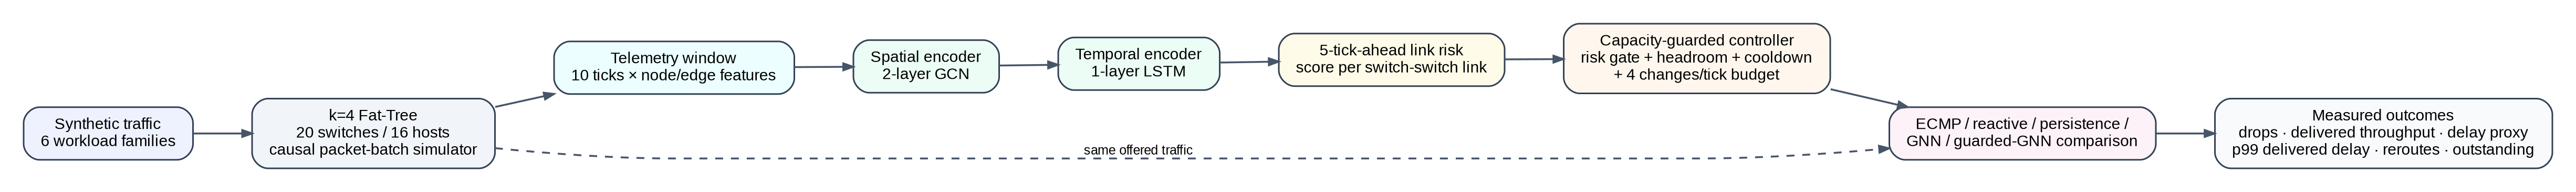
\includegraphics[width=0.92\textwidth]{research/system_architecture.png}
\caption{NeuralFabric pipeline used in the experiments. The implementation is a synthetic teaching/research simulator; telemetry is INT-style rather than packet-header-level INT, and route installation delay is not simulated.}
\label{fig:architecture}
\end{figure*}

\subsection{Synthetic Topology and Forwarding Model}
The default topology is a k=4 Fat-Tree containing 20 switches and 16 hosts. Switch-to-switch links have a nominal metadata value of 10 Gbps, a simulated capacity of 500 packets/tick, a 2000-packet buffer, and 0.5 microseconds of propagation metadata. The nominal Gbps value is not converted into packets/tick and is therefore not used as a calibrated physical serialization rate.

The simulator uses a 1 ms tick. Each physical link has one shared FIFO queue for both directions. Packets advance at most one link per tick. Source rates can be fractional; the simulator accumulates the fractional part until an integer number of packets is offered. Drops occur when a queue is full. For every run, the simulator asserts the accounting identity
\begin{equation}
P_{offered}=P_{dropped}+P_{delivered}+P_{outstanding}.
\end{equation}
This prevents duplicated or silently lost packets from masquerading as routing improvements.

\subsection{Traffic Families}
Six traffic generators are evaluated: uniform background flows, hotspot/incast traffic, elephant/mice mixtures, structured stride traffic, synthetic collective-inspired LLM-training bursts, and a mixed workload combining these generators. The LLM-training generator is explicitly synthetic; it does not execute NCCL, RoCEv2, or GPU communication and therefore should not be interpreted as a trace-replay workload.

\section{Congestion Forecasting Model}
\subsection{Telemetry Features and Label}
For each switch, the node feature vector is
\begin{equation}
\mathbf{x}^{node}=[q_{avg},t_{out},d,b],
\end{equation}
where queue occupancy, throughput, drops, and buffer usage are normalized by configured capacities. For each switch-to-switch edge, the edge feature vector is
\begin{equation}
\mathbf{x}^{edge}=[u,q,d,\ell],
\end{equation}
where $u$ is offered arrivals divided by capacity, $q$ is normalized queue depth, $d$ is normalized packet drops, and $\ell$ is a latency proxy normalized by 100 microseconds. The binary target is one when the raw offered utilization exceeds 0.85 at the future target tick.

A sample contains a $W=10$ tick history and predicts the target at $H=5$ ticks after the last observed feature. Windows are formed per scenario before splitting, and the split is performed by whole scenario IDs so overlapping windows cannot cross train, validation, and test partitions.

\subsection{GCN-LSTM}
For each observed timestep, the GCN encoder applies two layers of normalized graph convolution:
\begin{equation}
\mathbf{H}^{(l+1)}=\sigma(\hat{\mathbf{D}}^{-1/2}\hat{\mathbf{A}}\hat{\mathbf{D}}^{-1/2}\mathbf{H}^{(l)}\mathbf{W}^{(l)}),
\end{equation}
where self-loops are included in $\hat{\mathbf{A}}$ and $\sigma$ is followed by layer normalization, ReLU, and dropout. Source and destination node embeddings are concatenated with the edge features and projected into a 32-dimensional temporal representation. One LSTM layer processes each edge history, and a small multilayer perceptron followed by a sigmoid outputs a per-edge congestion score.

The model contains 17,985 trainable parameters and is trained using Adam with learning rate $10^{-3}$, weight decay $10^{-4}$, weighted binary cross-entropy with positive weight 3, gradient clipping at 1.0, and early stopping based on validation F1. The stored research checkpoint was produced with 20 training epochs in the recorded benchmark.

\subsection{Persistence Baseline}
To determine whether learning is necessary for the forecast task, a persistence baseline holds the last observed congestion label constant. This baseline is intentionally simple but important: a model should beat persistence on the forecast task before a routing gain is attributed to prediction quality.

\section{Capacity-Guarded Routing Controller}
The controller receives a per-edge forecast vector $p_e$ and uses the path risk
\begin{equation}
r(\pi)=\max_{e\in\pi}p_e.
\end{equation}
An active flow is considered only when its current path has risk above the alert threshold $\tau=0.7$. Candidate paths are generated as weighted simple paths, with edge cost increasing with predicted risk, and at most three alternatives are considered.

A candidate move must satisfy all of the following conditions: the predicted path risk must improve by at least $\delta=0.15$; hop count may increase by at most two; the flow must not be within its five-tick cooldown; the prediction must be no more than one tick old; and the global change budget of four moves per tick must not be exceeded.

Capacity is checked conservatively. For each physical link $e$, the controller initializes demand as the maximum of the sum of active-flow rates on that link and the current observed packet arrivals. A newly added link is admissible only if
\begin{equation}
D(e)+r_f+Q(e)\leq\alpha C(e),
\end{equation}
where $r_f$ is the moved flow rate, $Q(e)$ is queued packets, $C(e)$ is configured capacity, and $\alpha=0.90$ is the headroom factor. Accepted moves immediately reserve the new path and release the old-path demand before the next decision. Thus, multiple moves cannot independently assume the same untouched headroom.

The controller is not a bandwidth allocator in the physical sense. It is a conservative one-tick admission proxy designed for this simulator. It also has no RDMA ordering guarantee: packets that were already queued on an old path keep their original path while future packets may use the new path.

\section{Experimental Method}
The recorded research benchmark uses 30 generated data scenarios. Whole scenarios are grouped into train, validation, and test partitions: 21, 4, and 5 scenarios respectively. The predictor is trained once with a fixed seed on the recorded benchmark configuration. The routing study then uses three separate seeds (3000--3002) for each of the six workload families. Each seed is run under five matched strategies: ECMP, reactive rerouting, persistence-based routing, unguarded GNN rerouting, and capacity-guarded GNN rerouting. This yields 6$\times$3$\times$5=90 routing runs.

The predictor is evaluated using F1 at a 0.5 classification cutoff, average precision (AP), ROC AUC, and Brier score. Routing is evaluated using packet drops, delivered packets/tick, delivered-packet mean delay, mean per-run p99 delivered delay, outstanding packets, and reroute mutations. The p99 value is computed within each run from the tick-quantized delivered-packet delay distribution, then averaged across runs; it is not a pooled packet percentile.

Because only three traffic seeds are used per family and overlapping windows exist within held-out scenarios, all statistical intervals are treated as descriptive pilot evidence rather than definitive significance tests.

\section{Results}
\subsection{Forecast Quality}
Table~\ref{tab:prediction} shows that the GNN provides stronger ranking and probabilistic error metrics than persistence but not a higher F1 at the fixed 0.5 threshold. This is an important negative result: the GNN is not demonstrably necessary for the forecast task under this setup.

\begin{table}[t]
\centering
\caption{Held-out congestion forecast metrics across test-scenario windows.}
\label{tab:prediction}
\small
\begin{tabular}{lrrrr}
\toprule
Predictor & F1 & AP & ROC AUC & Brier\\
\midrule
GCN-LSTM & 0.7940 & 0.8692 & 0.9580 & 0.0676\\
Persistence & 0.8118 & 0.6991 & 0.8799 & 0.0777\\
\bottomrule
\end{tabular}
\end{table}

\begin{figure}[t]
\centering
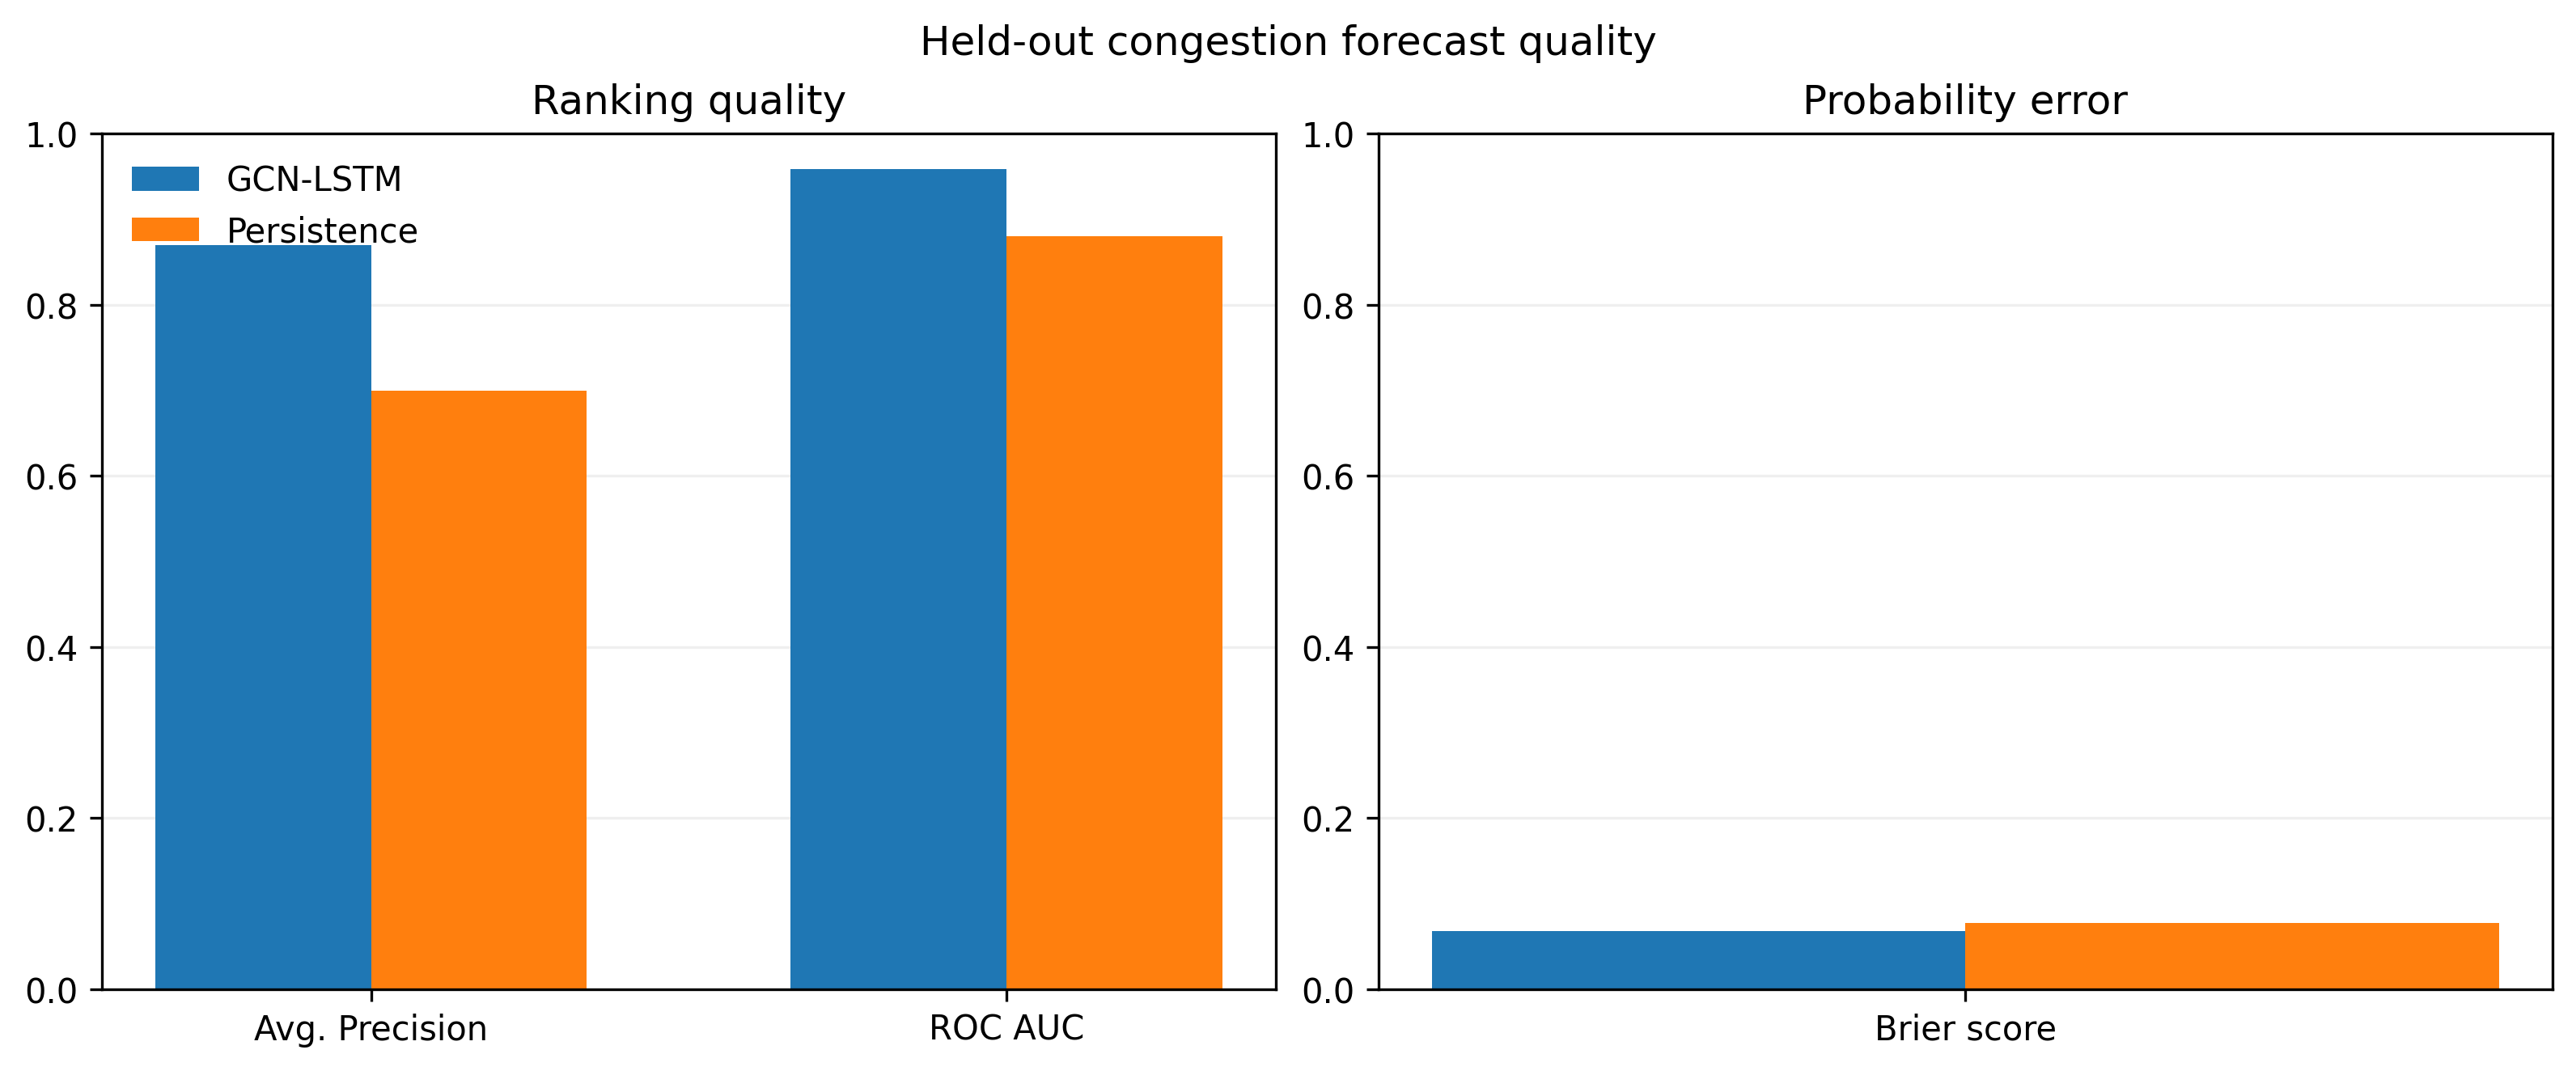
\includegraphics[width=0.48\textwidth]{research/metrics_chart.png}
\caption{Forecast ranking and probabilistic metrics from the recorded benchmark. Higher is better for F1, AP and ROC AUC; lower is better for Brier score.}
\label{fig:pred_metrics}
\end{figure}

\subsection{Packet Drops by Workload}
Table~\ref{tab:drops} reports mean packet drops per run across the three matched seeds in each family. Guarded GNN routing reduces ECMP drops in five families and ties it in the synthetic LLM-training family. The strongest improvement occurs for stride traffic (86.4\%). For the mixed workload the improvement is only 0.49\%, showing that a positive aggregate result can hide workload-specific weaknesses.

\begin{table*}[t]
\centering
\caption{Mean packet drops per run across matched seeds. Lower is better.}
\label{tab:drops}
\small
\begin{tabular}{lrrrrr}
\toprule
Traffic family & ECMP & Reactive & Persistence & GNN & Guarded GNN\\
\midrule
Uniform & 125,414 & 105,800 & 108,179 & 115,685 & \textbf{108,553}\\
Hotspot & 367,280 & 355,871 & 353,731 & 358,582 & 355,600\\
Elephant + mice & 120,190 & 100,818 & 99,822 & 100,162 & \textbf{98,349}\\
Stride & 59,840 & 18,250 & 20,099 & 35,397 & \textbf{8,113}\\
LLM-training & 32,291 & 32,239 & 32,228 & 32,214 & 32,291\\
Mixed & 1,105,914 & 1,109,953 & 1,098,154 & 1,122,231 & 1,100,487\\
\bottomrule
\end{tabular}
\end{table*}

\begin{figure}[t]
\centering
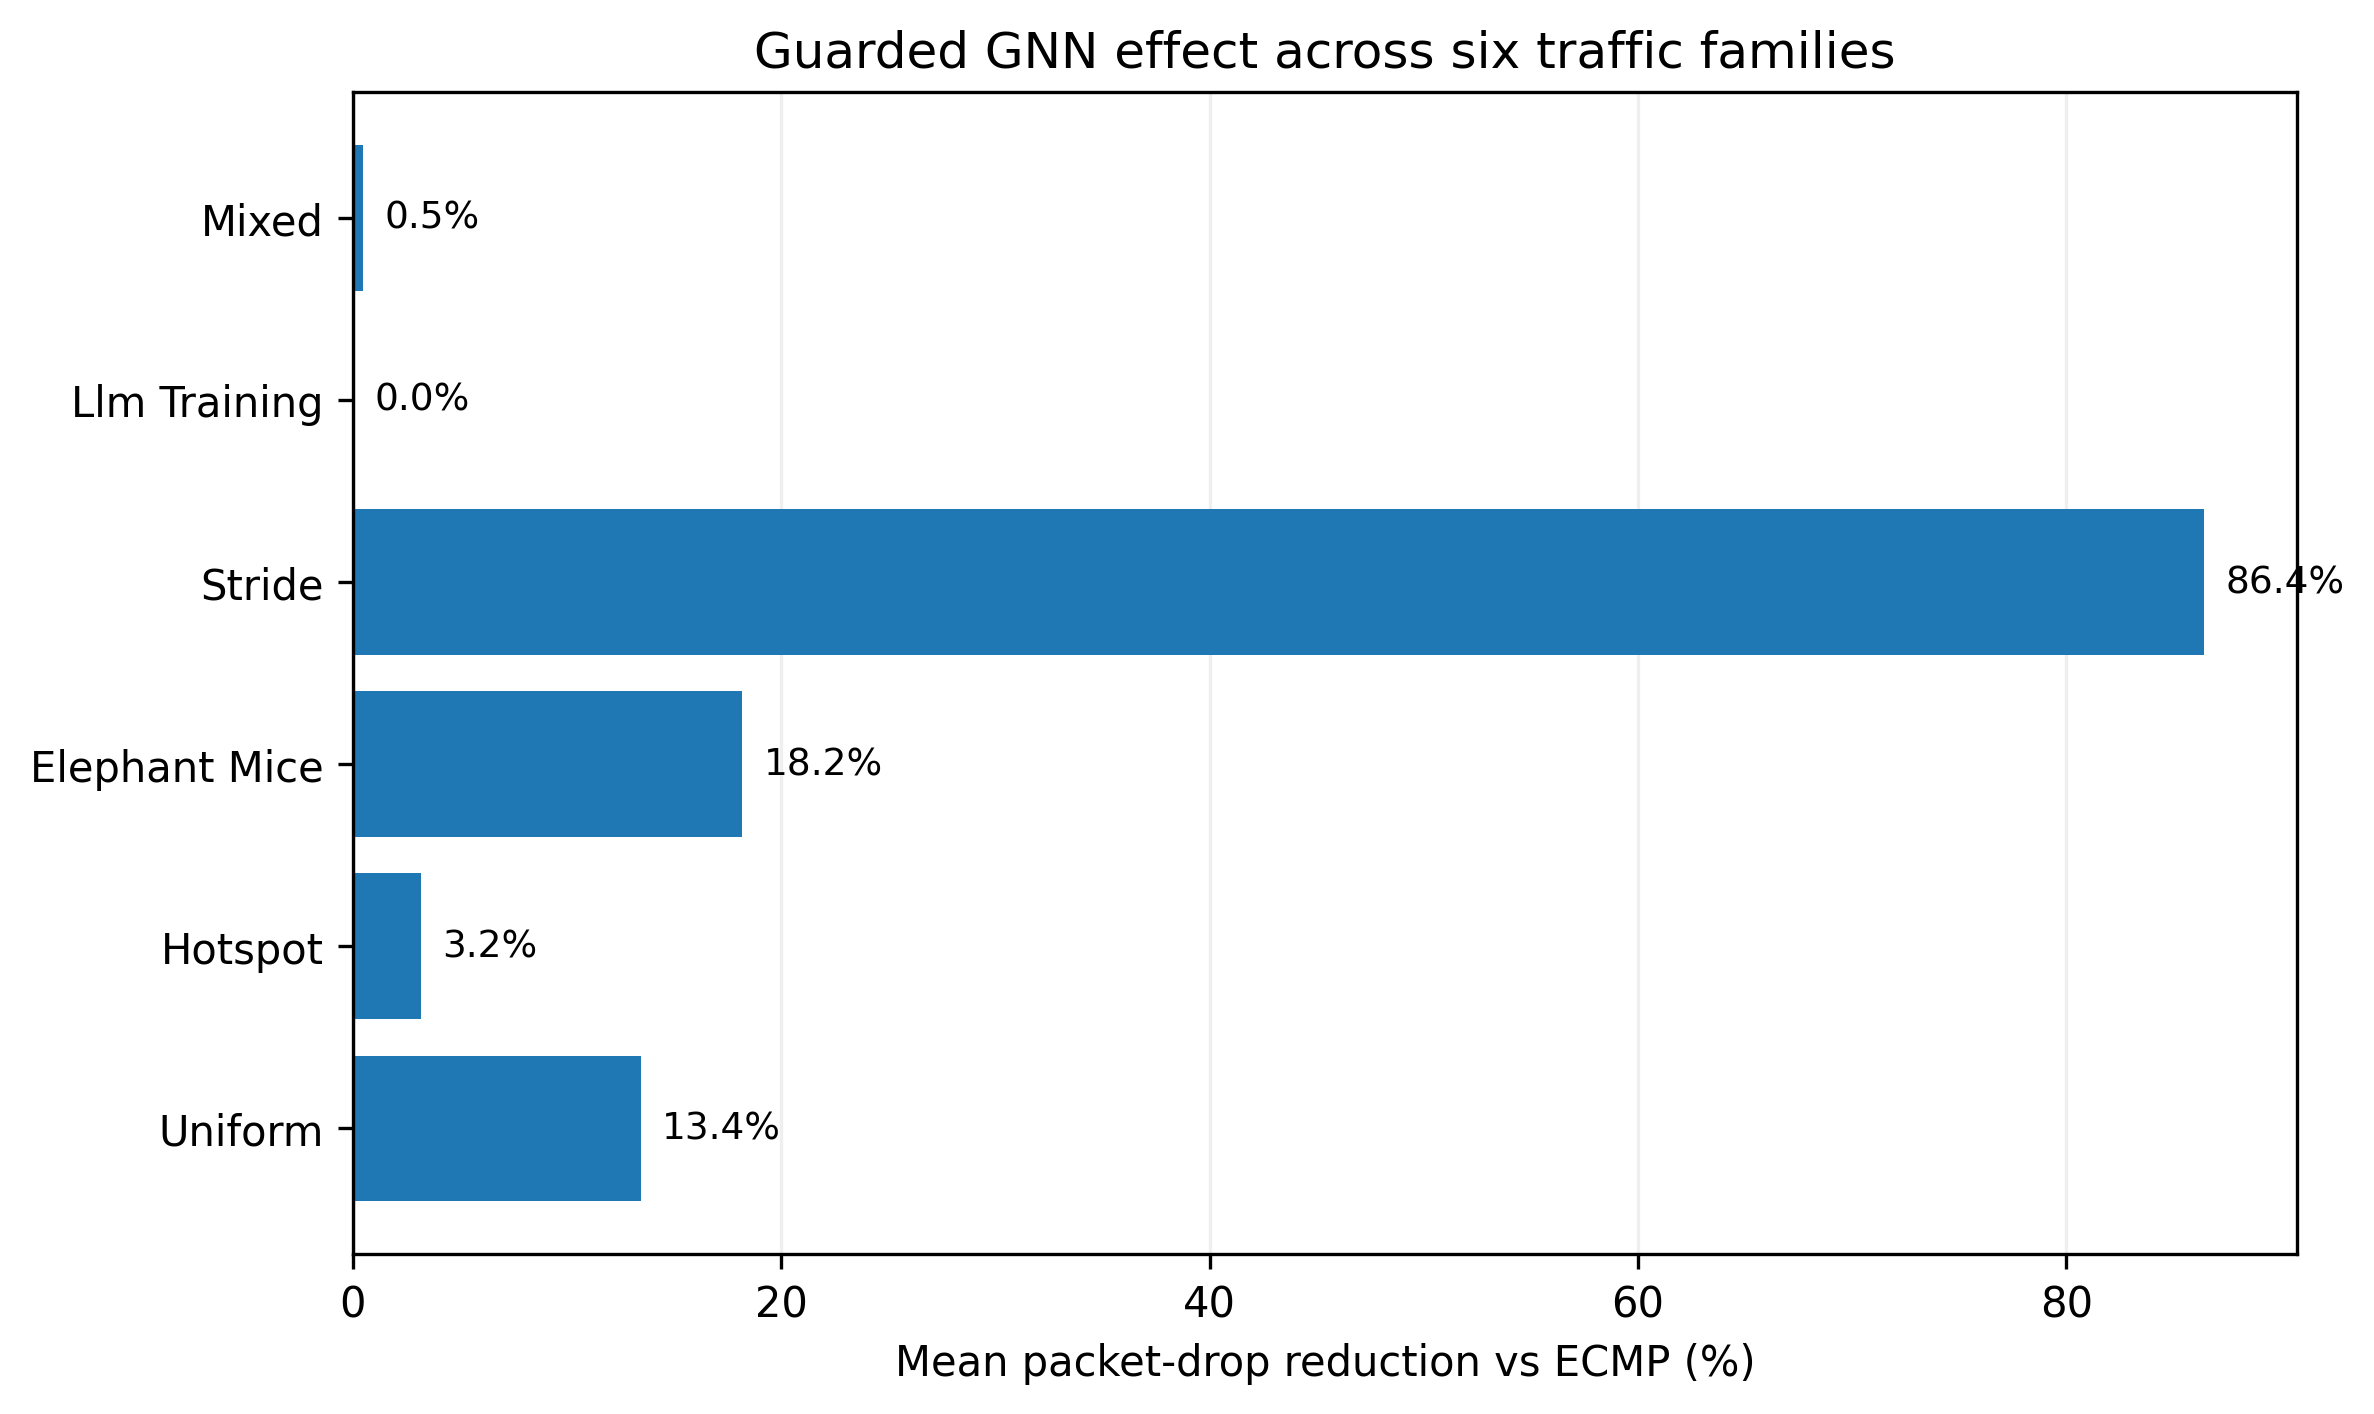
\includegraphics[width=0.48\textwidth]{research/drop_reduction.png}
\caption{Guarded GNN packet-drop reduction relative to ECMP for each synthetic traffic family.}
\label{fig:drop_reduction}
\end{figure}

\subsection{Overall Routing Outcomes}
Across the 18 matched traffic trials, the guarded controller has the lowest mean packet drops among the five strategies. It also has the highest mean delivered packets/tick and the lowest mean delivered delay among the recorded strategies, but these are simulator metrics rather than production network measurements. Table~\ref{tab:overall} provides the aggregate values.

\begin{table*}[t]
\centering
\caption{Overall mean routing outcomes across the 18 matched traffic trials.}
\label{tab:overall}
\small
\begin{tabular}{lrrrrr}
\toprule
Strategy & Drops/run & Delivered pkt/tick & Mean delivered delay (ms) & Mean run p99 (ms) & Reroutes/run\\
\midrule
ECMP & 301,821.5 & 1,852.28 & 9.664 & 17.389 & 0.00\\
Reactive & 287,155.1 & 1,944.11 & 10.606 & 22.944 & 622.83\\
Persistence & 285,368.7 & 1,958.91 & 10.497 & 22.000 & 613.94\\
GNN & 294,045.2 & 1,899.98 & 10.606 & 22.222 & 588.89\\
Guarded GNN & \textbf{283,899.0} & \textbf{1,979.47} & \textbf{9.008} & \textbf{15.889} & \textbf{14.72}\\
\bottomrule
\end{tabular}
\end{table*}

The guarded controller beats or ties ECMP on all 18 paired routing trials: 15 wins, 3 ties, and 0 losses. Its mean drop reduction relative to ECMP is 5.94\%. The mean reroute count is 14.72 per run, versus 622.83 for reactive rerouting, corresponding to a 97.6\% reduction in route mutations.

\begin{figure}[t]
\centering
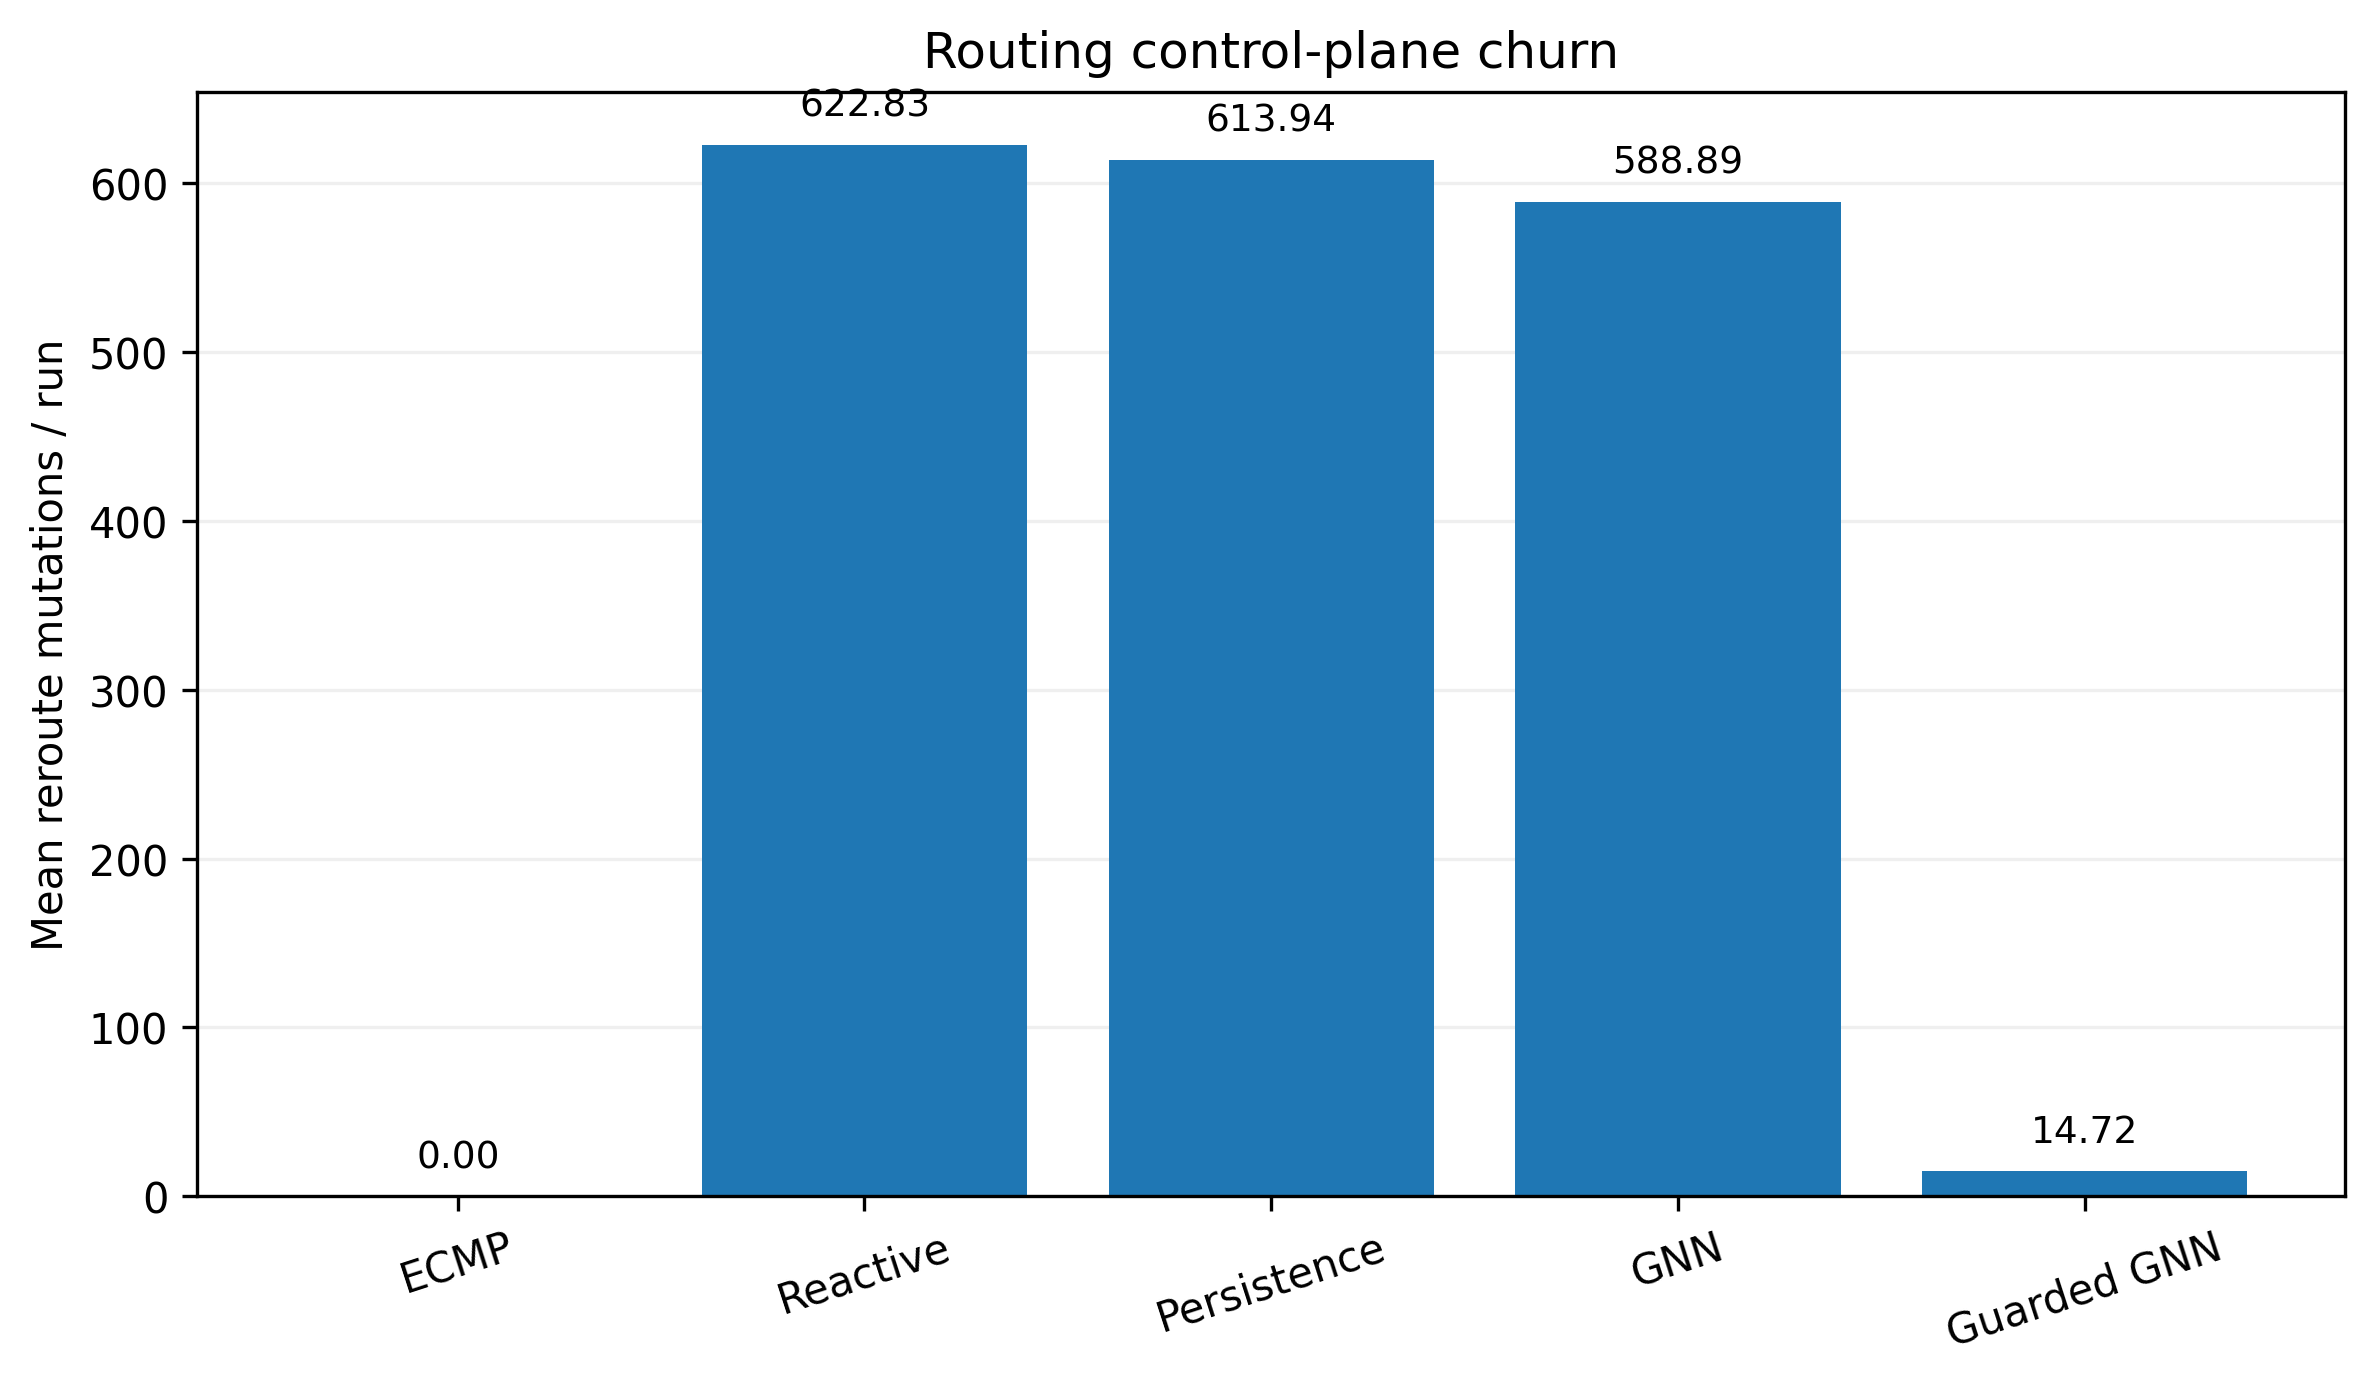
\includegraphics[width=0.48\textwidth]{research/reroutes_chart.png}
\caption{Mean route mutations per run. Guarded GNN sharply limits control-plane route changes relative to the unconstrained baselines.}
\label{fig:reroutes}
\end{figure}

\begin{figure}[t]
\centering
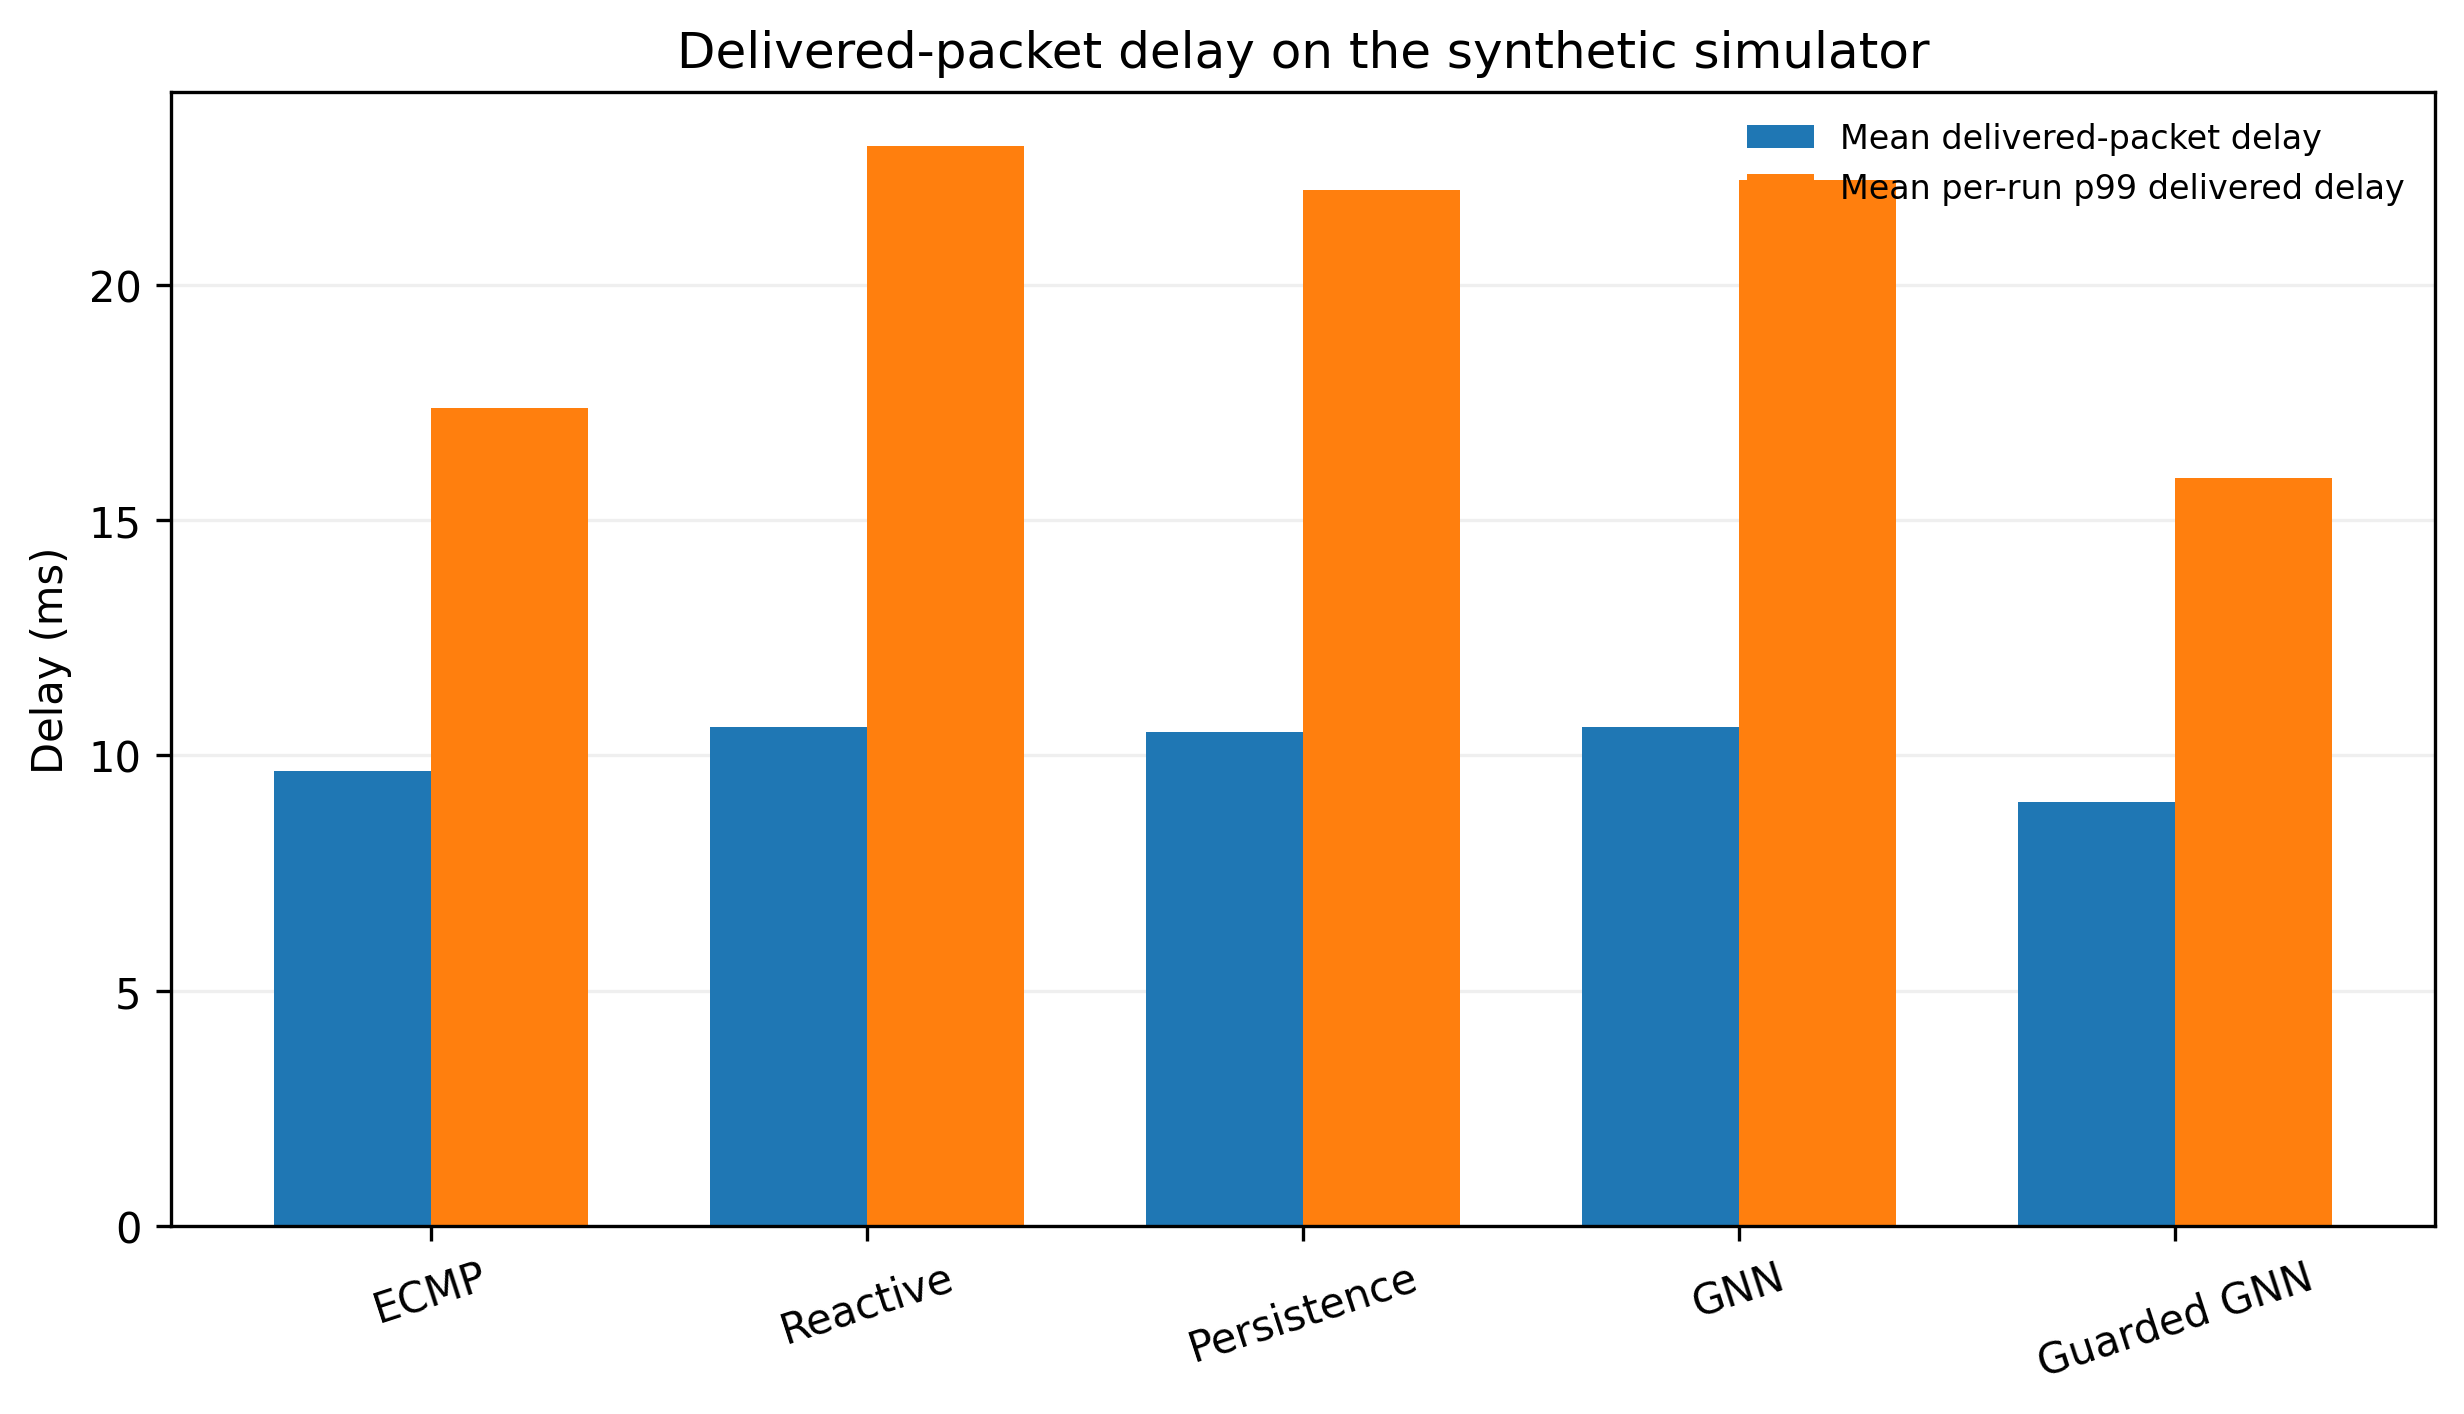
\includegraphics[width=0.48\textwidth]{research/latency_chart.png}
\caption{Mean delivered-packet delay by routing strategy. The values are tick-quantized simulator statistics, not measured network latency.}
\label{fig:latency}
\end{figure}

\section{Discussion}
The results support a narrower claim than the original project framing: in this simulator, a conservative admission controller can convert noisy forecast signals into fewer route changes while maintaining or improving several aggregate routing metrics. The controller's strongest effect is not simply predicting congestion; it is refusing moves that fail a capacity or policy check. The persistence baseline is a useful reminder that the forecast model and the routing controller should be evaluated separately.

The stride workload is especially favorable because its structured traffic creates repeatable pressure on a subset of shortest paths. The guarded controller can exploit alternate capacity in that setting. In contrast, hotspot and destination-incast traffic can create a bottleneck at the destination or its adjacent links that routing alone cannot remove. The mixed workload also shows that small average improvements are possible even when the unguarded GNN is worse than simpler baselines.

The 97.6\% reduction in route mutations is a meaningful control signal in this prototype, but it should not be interpreted as proof that the controller prevents route flapping in RDMA hardware. The simulator does not model transport acknowledgements, sequence numbers, packet reordering, switch programming delay, or PFC pause propagation. Those mechanisms can materially change the cost of a route change.

\subsection{Inference Time}
The recorded benchmark reports per-inference p99 values between 6.185 and 13.516 ms on the host used for the experiment. These measurements exclude telemetry export, path computation, and route installation, and the simulator does not wait for inference to complete. Because the forecast horizon is 5 ms, some observed inference tails exceed the horizon. Therefore, the current timing is an implementation diagnostic, not evidence that the system can react inside a real datacenter control loop.

\section{Threats to Validity}
\textbf{Simulation abstraction:} the network engine is a causal packet-batch model, not a packet-level implementation of Ethernet, RoCEv2, PFC, ECN, DCQCN, or NCCL.

\textbf{Traffic realism:} the six traffic families are synthetic generators. The LLM-training family is collective-inspired rather than trace driven, and no production workload calibration is claimed.

\textbf{Topology scope:} all runs use a single k=4 Fat-Tree size. Generalization to other topologies is untested.

\textbf{Statistical power:} the routing study has only three seeds per family, and forecast windows overlap within a scenario. Bootstrap intervals in the project files are therefore descriptive only.

\textbf{Model and controller coupling:} the routing threshold, capacity guard, and change budget were fixed configuration choices rather than selected through a large independent hyperparameter sweep. The GNN is also trained with a single recorded training seed.

\textbf{Timing and ordering:} a 1 ms tick cannot establish microsecond response behavior. Current packets retain their old routes after a flow change, so packets can traverse different paths without any RDMA ordering model.

\section{Reproducibility and Project Artifacts}
All reported routing results are stored as structured records in \texttt{research/benchmark\_results.json}. The project includes a requirements file for the tested environment, the trained checkpoint, generated datasets, unit/integration tests, and scripts for data generation, training, evaluation, and benchmark reproduction. The checkpoint loader accepts both PyTorch Geometric and bundled manual-GCN state-dict layouts, improving portability across environments.

A clean reproduction should install the tested dependency versions, run the 13 regression/integration tests, and then execute \texttt{research\_benchmark.py} with the recorded benchmark settings. Reproducing the exact wall-clock inference timing still depends on hardware, operating-system load, and library versions.

\section{Limitations and Future Work}
The next technical step is not to add more marketing claims but to close the simulation-to-system gap. A stronger study should evaluate at least 10--20 independent traffic seeds per family, multiple training seeds, several topology sizes, and explicit controller-delay sweeps. The routing policy should also be tested against a packet-level simulator with realistic full-duplex links, ECN/PFC or an equivalent lossless mechanism, transport dynamics, packet ordering, and rule-installation delay. Hardware or SmartNIC/P4 measurements would then be needed before making any deployment-time claim.

On the modelling side, future work should compare the GCN-LSTM against stronger non-neural predictors, calibrate probability outputs, tune the controller threshold on validation data rather than by fixed convention, and report confidence intervals over independent runs. A useful ablation would separately remove the capacity guard, route-change budget, cooldown, and minimum-improvement gate to quantify their individual effects.

\section{Conclusion}
NeuralFabric is best viewed as a reproducible experimental study of capacity-guarded predictive routing. The recorded 90-run benchmark shows a 5.94\% mean reduction in packet drops versus ECMP, 15 wins and 3 ties across matched trials, an 86.4\% reduction for the structured stride workload, and a 97.6\% reduction in route mutations versus reactive rerouting. At the same time, the GNN does not beat persistence on F1, the mixed workload benefit is small, and the simulator does not represent PFC, RDMA, or a real-time control loop. Those limitations are part of the result. The main conclusion is therefore that forecast-driven rerouting becomes more defensible when forecast actions are subject to explicit capacity and stability guards, while substantial additional experimental work is required before broader claims can be made.

\begin{thebibliography}{00}

\bibitem{benson2010network}
T.~Benson, A.~Akella, and D.~A.~Maltz, ``Network traffic characteristics of data centers in the wild,'' in \emph{Proc. 10th ACM Internet Measurement Conference}, 2010, pp.~267--280.

\bibitem{alfares2008}
M.~Al-Fares, A.~Loukissas, and A.~Vahdat, ``A scalable, commodity data center network architecture,'' in \emph{Proc. ACM SIGCOMM}, 2008, pp.~63--74.

\bibitem{hopps2000}
C.~Hopps, ``Analysis of an equal-cost multi-path algorithm,'' RFC~2992, IETF, 2000.

\bibitem{alizadeh2014conga}
M.~Alizadeh, T.~Edsall, S.~Dharmapurikar, R.~Vaidyanathan, K.~Chu, A.~Fingerhut, V.~T.~Lam, F.~Matus, R.~Pan, and L.~Vigoda, ``CONGA: Distributed congestion-aware load balancing for datacenters,'' in \emph{Proc. ACM SIGCOMM}, 2014, pp.~503--514.

\bibitem{katta2016hula}
N.~Katta, M.~Hira, C.~Kompella, A.~Vahdat, and J.~Rexford, ``HULA: Scalable load balancing using programmable data planes,'' in \emph{Proc. ACM Symposium on SDN Research}, 2016.

\bibitem{rusek2020routenet}
K.~Rusek, J.~Su{\'a}rez-Varela, P.~Almasan, P.~Barlet-Ros, and A.~Cabellos-Aparicio, ``RouteNet: Leveraging graph neural networks for network modeling and optimization in software-defined networks,'' \emph{IEEE Journal on Selected Areas in Communications}, vol.~38, no.~10, pp.~2260--2270, 2020.

\bibitem{ferriol2023routnetfermi}
M.~Ferriol-Galm\'es \emph{et al.}, ``RouteNet-Fermi: Network modeling with graph neural networks,'' \emph{IEEE/ACM Transactions on Networking}, 2023.

\bibitem{li2019hpcc}
Y.~Li \emph{et al.}, ``HPCC: High precision congestion control,'' in \emph{Proc. ACM SIGCOMM}, 2019, pp.~44--58.

\bibitem{benbasat2020pint}
R.~Ben Basat \emph{et al.}, ``PINT: Probabilistic in-band network telemetry,'' in \emph{Proc. ACM SIGCOMM}, 2020.

\bibitem{bernardez2025graphcc}
G.~Bern\'ardez, J.~Su{\'a}rez-Varela, X.~Shi, S.~Xiao, X.~Cheng, P.~Barlet-Ros, and A.~Cabellos-Aparicio, ``GraphCC: A practical graph learning-based approach to congestion control in datacenters,'' \emph{Computer Networks}, vol.~257, art.~110981, 2025, doi: 10.1016/j.comnet.2024.110981.

\bibitem{zhang2025ntpint}
P.~Zhang, H.~Zhang, Y.~Dai, C.~Zeng, J.~Wang, and J.~Liao, ``NTP-INT: Network traffic prediction-driven in-band network telemetry for high-load switches,'' \emph{Journal of Network and Computer Applications}, vol.~242, art.~104265, 2025, doi: 10.1016/j.jnca.2025.104265.

\bibitem{ahmad2026routnettg}
S.~Ahmad, G.~Srinivasa Rao, H.~A.~M.~Abdeljaber, E.~S.~N.~Joshua, F.~A.~Abdalla, and H.~Gadi, ``RouteNet-TGNN: A temporal graph neural network for delay and loss forecasting in dynamic communication networks,'' \emph{Journal of Communications}, vol.~21, no.~2, pp.~211--225, 2026, doi: 10.12720/jcm.21.2.211-225.

\bibitem{zhu2015dcqcn}
Y.~Zhu \emph{et al.}, ``Congestion control for large-scale RDMA deployments,'' in \emph{Proc. ACM SIGCOMM}, 2015, pp.~523--536.

\bibitem{hopper2025}
``Hopper: Congestion-aware path selection for load balancing in AI clusters,'' arXiv:2506.08132, 2025.

\bibitem{hu2025flb}
J.~Hu \emph{et al.}, ``Fine-grained load balancing in RDMA networks,'' in \emph{Proc. USENIX Annual Technical Conference (ATC)}, 2025.

\end{thebibliography}

\end{document}
